\section{Module 2: Lecture 4\\Decomposition of Signals}

\subsection{Introduction}
\noindent
 A fundamental idea in the study of signals is to represent signals in terms of linear combination of \textit{basis} signals. In the previous section, we have embarked on some important concepts, relating to the idea of representing signals as a linear combination of sinusoids.
 %In this lecture, we will be recapitulating those ideas.
We assumed that we wish to look either at periodic signals or signals over a finite interval $T$. Without loss of generality, let that interval be $(0,T)$. 

\noindent
We have assumed that such signals are signals spanned by  all sinusoids of angular frequency $\Omega = \frac{2\pi}{T}kt,k=0, \pm1, \pm2 ..$

\noindent
The typical periodic function, with period $T$ is of the form
\begin{equation*}
  x(t) = \sum_{k=-\infty}^{\infty} \! A_k\cos (\frac{2\pi}{T}kt + \phi_k)
\end{equation*}
where $A_k$ denotes the amplitude, $\Omega = \frac{2\pi}{T}k$ is the angular frequency and $\phi_k$ the phase.
We had proved that these sinusoids are orthogonal if they don’t have same angular frequency.
\begin{equation*}
  \langle A_{k_1} \cos (\frac{2\pi}{T}k_1t + \phi_1),A_{k_2} \cos (\frac{2\pi}{T}k_2t + \phi_2)\rangle = 0 \enspace \enspace \text{for} \enspace k_1 \neq k_2 
\end{equation*}

\noindent
This important concept requires appreciating several different ideas. Using these ideas, we can decompose signal $x(t)$ in terms of sinusoids. However, there are some signals which can’t be spanned using these sinusoids. Such signals are beyond the scope of discussion that we are going to undertake at this stage.
%%%
%%%
\subsection{ Orthogonal vectors at a particular frequency}
\noindent
Consider a periodic signal $x(t)$ with fundamental period $T$. Then we can write $x(t)$ as
%Let us assume the signal $x(t)$ as
\begin{equation*}
  x(t) = \sum_{k=-\infty}^{\infty} \! A_k\cos (\frac{2\pi}{T}kt + \phi_k)
\end{equation*}
%where $x(t)$ is periodic with period $T$ and w
We constrain ourselves to $0<t<T$.

\noindent
To calculate $A_k$ and $\phi_k$ we need to use the following property i.e.
\begin{equation*}
\langle \cos (\frac{2\pi}{T}k_1t + \phi_1), \cos (\frac{2\pi}{T}k_2t + \phi_2) \rangle = 0 \enspace \enspace		for \enspace k_1 \neq k_2 \end{equation*}

\noindent
We can think of the cosines $\cos (\frac{2\pi}{T}kt + \phi_k)$ as countably infinite orthogonal vectors, indexed by $k$, for $k=0, \pm1, \pm2...$ and so on.

\noindent
To find out the component of $x(t)$ along these orthogonal vectors, we need to take the dot product of $x(t)$ with the unit vector, in the direction of orthogonal vectors $\cos(\frac{2\pi}{T}kt + \phi_k), 0<t<T$.
For calculating unit vector, we need to find the magnitude of the vector $\cos(\frac{2\pi}{T}kt + \phi_k)$ using dot product.

\begin{align*} \left|\cos(\frac{2\pi}{T}kt + \phi_k)\right| &= \langle \cos (\frac{2\pi}{T}kt + \phi_k), \cos (\frac{2\pi}{T}kt + \phi_k)\rangle \\
  &= \int_{0}^{T} \! \cos (\frac{2\pi}{T}kt + \phi_k) \cos (\frac{2\pi}{T}kt + \phi_k) \ \dm t \\
  &= \int_{0}^{T} \! \cos^2 (\frac{2\pi}{T}kt + \phi_k) \ \dm t \\
  &= \int_{0}^{T} \! (\frac{1}{2} + \cos (2(\frac{2\pi}{T}kt + \phi_k)) \ \dm t \\
  &= \int_{0}^{T} \! \frac{1}{2} \ \dm t + \int_{0}^{T} \! \cos (2(\frac{2\pi}{T}kt + \phi_k)) \ \dm t \\
  &= \frac{T}{2}
\end{align*}
%%%
Thus, the magnitude square of the cosine is $T/2$ and hence the magnitude is $\sqrt{T/2}$. So, the unit vector is given by

\begin{equation*} \textrm{Unit vector} = \sqrt{\frac{2}{T}}\cos (\frac{2\pi}{T}kt + \phi_k)\end{equation*}
                    
\noindent
But still, there is one unknown quantity, namely, $\phi_k$ in this unit vector. However, we can think of this vector as a vector in a two dimensional space:

\begin{equation*}\sqrt{\frac{2}{T}}\cos (\frac{2\pi}{T}kt + \phi_k) = \sqrt{\frac{2}{T}}[\cos\phi_k\cos (\frac{2\pi}{T}kt) - \sin\phi_k\sin (\frac{2\pi}{T}kt)] \end{equation*}
that is, the unit vector can be thought of as a linear combination of two vectors.

\noindent
We have,
\begin{align*}
  \langle \cos (\frac{2\pi}{T}kt + \phi_k), \sin (\frac{2\pi}{T}kt + \phi_k) \rangle &= \int_{0}^{T} \! \cos (\frac{2\pi}{T}kt + \phi_k) \sin (\frac{2\pi}{T}kt + \phi_k) \ \dm t  \\
  &= \frac{1}{2} \int_{0}^{T} \! 2 \cos (\frac{2\pi}{T}kt + \phi_k) \sin (\frac{2\pi}{T}kt + \phi_k) \ \dm t \\
  &= \frac{1}{2} \int_{0}^{T} \! \sin (\frac{4\pi}{T}kt + \phi_k) \ \dm t \\
  &= 0
\end{align*}
%%%
Hence, the cosine and sine components are also orthogonal. $\cos\phi_k$ and $\sin\phi_k$ are now two unknown constants.
%%%
Therefore, decomposing $x(t)$ along $\cos (\frac{2\pi}{T}kt + \phi_k)$ will give the same results as decomposing $x(t)$ along  $\cos (\frac{2\pi}{T}kt)$ and $\sin (\frac{2\pi}{T}kt)$. So, to decompose $x(t)$ along $\cos (\frac{2\pi}{T}kt)$ and $\sin (\frac{2\pi}{T}kt)$, we require unit vectors, which we already have calculated above.
%%%
So, the two unit vectors are $\sqrt{\frac{2}{T}}\cos (\frac{2\pi}{T}kt)$ and $\sqrt{\frac{2}{T}}\sin (\frac{2\pi}{T}kt)$.
%%%
%%% 
\subsection{Projection of Vectors}
Let $u_1$ = $\sqrt{\frac{2}{T}}\cos (\frac{2\pi}{T}kt)$ and $u_2 = \sqrt{\frac{2}{T}}\sin (\frac{2\pi}{T}kt)$. We know that at frequency $2\pi k/T$, there are two orthogonal vectors, $u_1$ and $u_2$. We have a two dimensional space and we need to calculate the component of the vector $x(t)$ along orthogonal vectors of this 2D space.
  
\noindent
 Let $v$ be any arbitrary vector of higher dimension and $v_p$ be the projection of $v$ onto our 2D space spanned by orthogonal vectors $u_1$ and $u_2$. To calculate the components of the vector $v$ along the two orthogonal vectors, we can project $v_p$  onto $u_1$ and $u_2$. We can also directly project $v$ onto $u_1$ and $u_2$.
 


\noindent
 The vector $v$ can be written as $v = v_p  + v_\perp$, where $v_p$ is the projection of $v$ on to 2D space and $v_\perp$ is component perpendicular to the 2D space . The projection of $v$ onto vectors $u_1$ and $u_2$ will be same as the projection of $v_p$  on those vectors, as the $v_\perp$ will not contribute in projection.
 
\begin{figure}[ht]
\centering
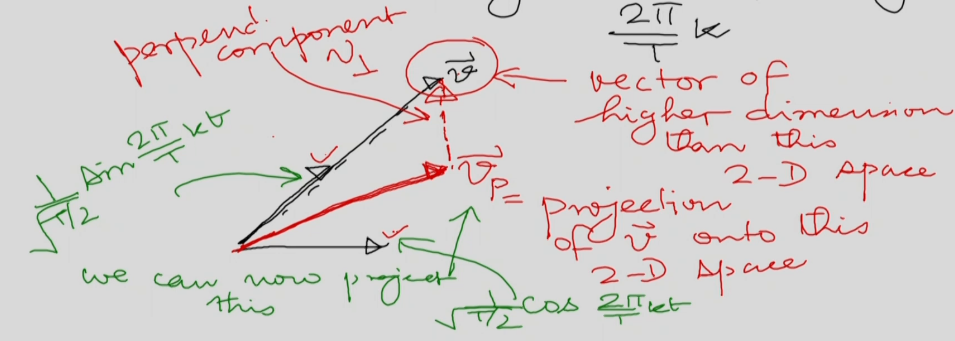
\includegraphics[scale=0.32]{S_215.PNG}		
\end{figure}

 \begin{figure}[ht]
\centering
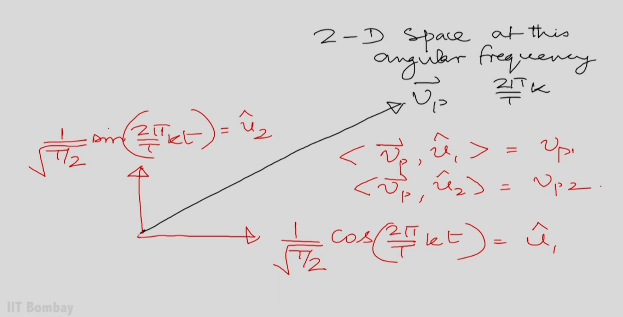
\includegraphics[scale=0.32]{S_215_2.PNG}		
\end{figure}

\noindent
Let us project $v_p$ along the two orthogonal vectors. 
  For projecting  $v_p$  along $u_1$ and $u_2$, taking dot product 
 
\begin{equation*} \langle v_p, u_1 \rangle =v_{p_1} \end{equation*}
\begin{equation*} \langle v_p, u_2 \rangle = v_{p_2} \end{equation*}
 
\noindent
$v_p$  in terms of $u_1$, $u_2$ can be written as $v_p$  = $v_{p_1}u_1$ + $v_{p_2}u_2$. Interestingly  $\langle v_p, u_1 \rangle = \langle v, u_1 \rangle$ is true also for $u_2$ as the perpendicular component $v_\perp$ is not going to contribute in the dot product. 
        
We know that the $k^{th}$ angular frequency =  $2 \pi k/T$.
At this frequency we have two components 
\begin{equation*}x(t) = \langle x(t), \sqrt{\frac{2}{T}}\cos (\frac{2\pi}{T}kt)\rangle \cdot \sqrt{\frac{2}{T}}\cos (\frac{2\pi}{T}kt) + \langle x(t), \sqrt{\frac{2}{T}}\sin (\frac{2\pi}{T}kt)\rangle \cdot \sqrt{\frac{2}{T}}\sin (\frac{2\pi}{T}kt)\end{equation*}
This can be simplified as

\begin{equation*}x(t) = \langle x(t), \cos (\frac{2\pi}{T}kt)\rangle \cdot \frac{2}{T}\cos (\frac{2\pi}{T}kt) + \langle x(t), \sin (\frac{2\pi}{T}kt)\rangle \cdot \frac{2}{T}\sin (\frac{2\pi}{T}kt)\end{equation*}

\noindent
\subsection{Decomposition of square wave}
We have a periodic signal $x(t)$ in Fig.\ref{fig:square-wave}, defined as
\[
x(t) =
\left\{
	\begin{array}{ll}
		1  & \mbox{if } 0 < t < \frac{T}{2} \\
		-1 & \mbox{if } \frac{T}{2} < t < T
	\end{array}
\right.
 \]

\noindent
$x(t) = x(t+T)$ for all $t$, i.e. $x(t)$ is periodic with period $T$.
              
\begin{figure}[ht]\label{fig:square-wave}
\centering
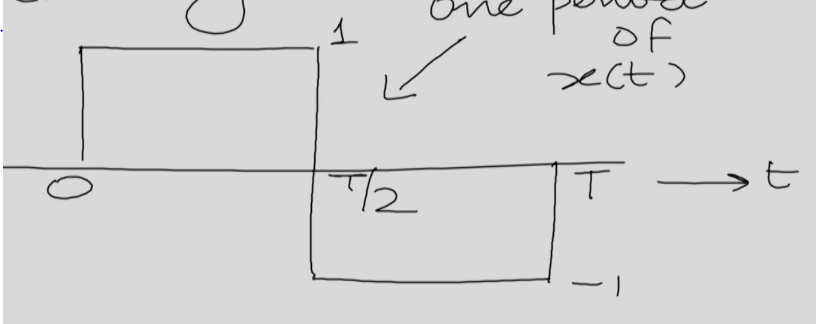
\includegraphics[scale=0.32]{S_216_1.PNG} %\\Figure 1
\caption{Plot of $x(t)$}
\end{figure}




\noindent
The zero frequency component is the  mean of $x(t)$ over a period $T$ which is $0$ since the net area under $x(t)$ in one period is zero.

\noindent
Let us calculate the quantity $\langle x(t), \cos (\frac{2\pi}{T}kt)\rangle \cdot \frac{2}{T}\cos (\frac{2\pi}{T}kt))$,


\noindent
For $k=1$ and $k=2$, we can see from Fig.\ref{fig:square-dot-cosine} that, the positive portion gets annulled by the negative portion. Similar is the case for $k=3, 4...$ and so on. Hence $\langle x(t), \cos (\frac{2\pi}{T}kt)\rangle= 0$ for given $x(t)$.


\begin{figure}[ht]\label{fig:square-dot-cosine}
\centering
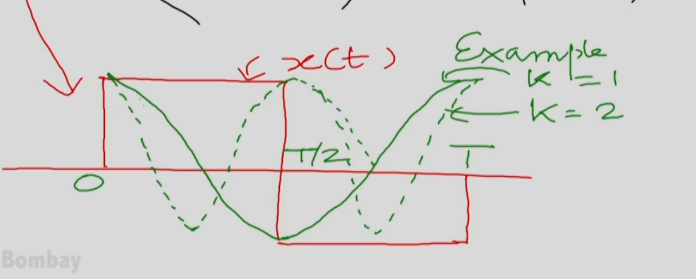
\includegraphics[scale=0.32]{s_216.PNG} %\\Figure 2
\caption{Dot product of the square wave with cosines}	
\end{figure}

\noindent
Calculating  $\langle x(t), \sin (\frac{2\pi}{T}kt)\rangle \cdot \frac{2}{T}\sin (\frac{2\pi}{T}kt)$, we have as shown in Fig.\ref{fig:square-dot-sine},

\begin{figure}[ht]\label{fig:square-dot-sine}
\centering
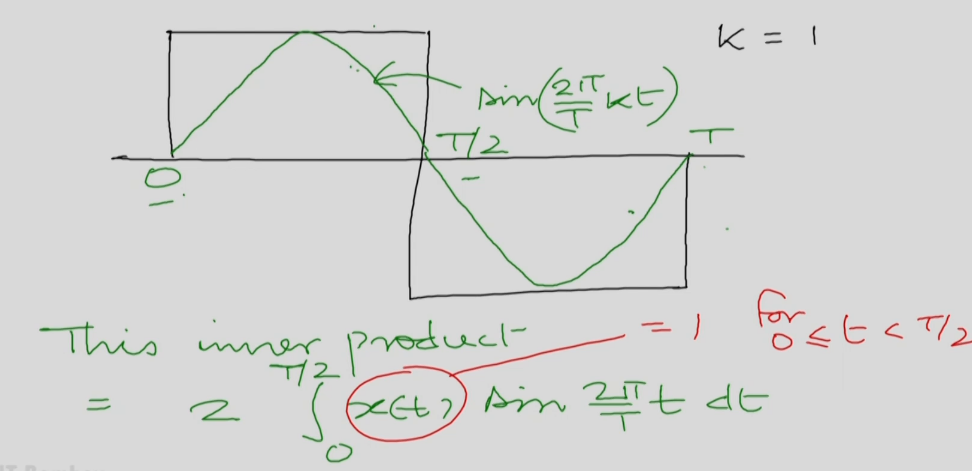
\includegraphics[scale=0.32]{S_216_3.PNG} %\\Figure 3
\caption{Dot product of the square wave with sines}	
\end{figure}
%%%
\begin{equation*} \langle x(t), \sin (\frac{2\pi}{T}kt)\rangle = \int_{0}^{T} \! x(t)\sin (\frac{2\pi}{T}kt) \ \dm t\end{equation*}
\begin{equation*} \langle x(t), \sin (\frac{2\pi}{T}kt)\rangle = \int_{0}^{\frac{T}{2}} \! \sin (\frac{2\pi}{T}kt) \ \dm t + \int_{\frac{T}{2}}^{T} \! {-\sin (\frac{2\pi}{T}kt)} \ \dm t \end{equation*}
\noindent
Also, we know that 
 \begin{equation*}\int_{0}^{\frac{T}{2}} \! \sin (\frac{2\pi}{T}kt) \ \dm t = -\int_{\frac{T}{2}}^{T} \! \sin (\frac{2\pi}{T}kt) \ \dm t \end{equation*}
\noindent
Using this, we have
\begin{equation*} \langle x(t), \sin (\frac{2\pi}{T}kt)\rangle = 2\int_{0}^{\frac{T}{2}} \! \sin (\frac{2\pi}{T}kt) \ \dm t = \left[-2\frac{\cos (\frac{2\pi}{T}kt)}{\frac{2\pi}{T}k}\right]_0^\frac{T}{2}\end{equation*}
%%%
For $k = 2n$, the above integral goes to zero as $\cos ({2\pi}n) = 1$ for all $n \in \mathbb{Z}$.
For $k = 2n-1$, the above integral has the value of $4T/\pi k$ because $\cos(2{\pi}(2n-1)) = -1$ for all $n \in \mathbb{Z}$. Thus,

\begin{equation*} \langle x(t), \sin (\frac{2\pi}{T}kt)\rangle = \frac{4T}{{\pi}k} \textrm{ (for odd }k) \end{equation*}
\noindent
Hence, we have, after multiplying by $2/T$,
\begin{equation*} x(t) = \sum_{n=1}^{\infty}\ \frac{4}{{\pi}(2k-1)} \sin (\frac{2\pi}{T}(2k-1)t)\end{equation*} 

\subsection{Examples of Decomposition}
\subsubsection{Exercise 1} 
\noindent
Work out the decomposition for an asymmetric square wave, of period $T$ as shown in the figure below.
\begin{figure}[ht]
\centering
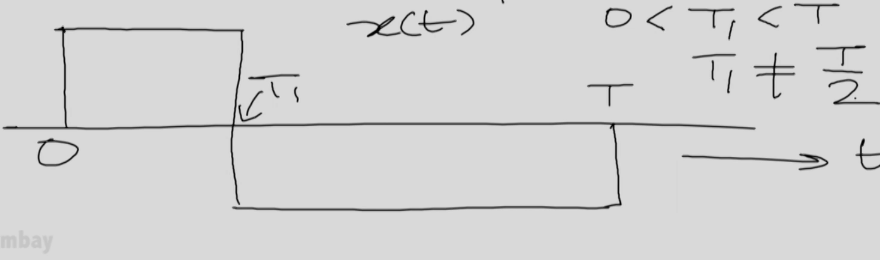
\includegraphics[scale=0.32]{S_217_1.PNG}
\end{figure}
 				\begin{equation*} x(t) = 1 \enspace \enspace      0<t<T_1 \end{equation*}
       			\begin{equation*} x(t) = -1  \enspace\enspace 	T_1 < t< T \end{equation*} \begin{equation*}0<T_1<T, \enspace T1\neq T/2, x(t+T) = x(t)\enspace  \forall t\in R.  \end{equation*}

                
\subsubsection{Exercise 2}
\noindent
In the answer of exercise 1 put $T_1 =T/2$, and verify the answer with that of decomposition of symmetric square wave.

\subsubsection{Exercise 3}
\noindent
Work out the decomposition for symmetric triangular wave, periodic with period $T$.

\noindent
\textit{Hint}: Use and observe the symmetry graphically.
\begin{figure}[ht]
\centering
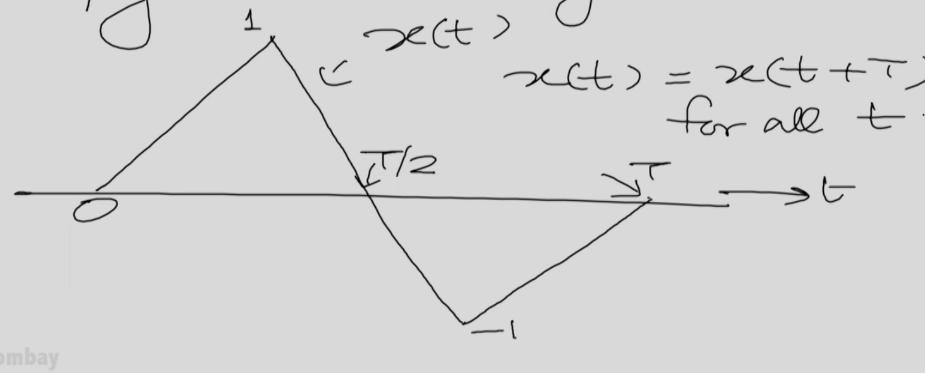
\includegraphics[scale=0.32]{S_217_2.PNG}
\end{figure}


\subsubsection{Exercise 4}
\noindent
Evaluate the decomposition for an asymmetric triangular wave as shown in the figure. Cross check the answer with that of exercise 3, by putting  $T_1 = T/2$ in the final answer.
\begin{figure}[ht]
\centering
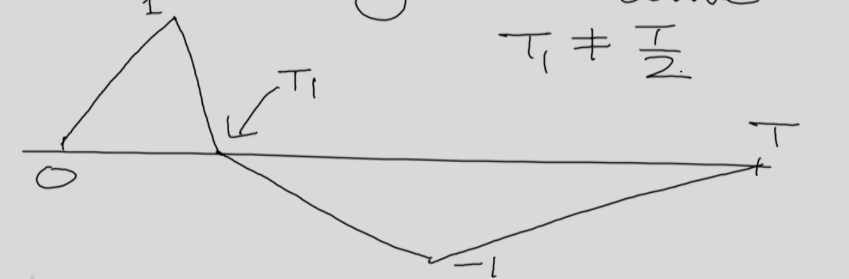
\includegraphics[scale=0.32]{S_217_3.PNG}
\end{figure}


\subsubsection{Exercise 5}
\noindent
A variant of symmetric triangular wave is shown below. Find its decomposition and compare with answer of exercise 3.
\begin{figure}[ht]
\centering
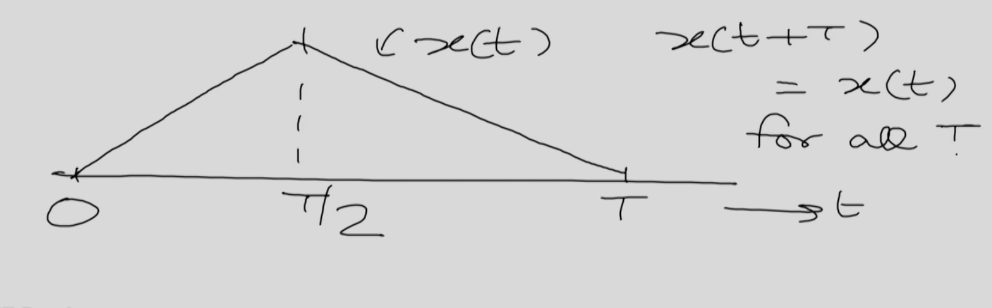
\includegraphics[scale=0.32]{S_217_4.PNG}
\end{figure}

\pagebreak

\subsubsection{Exercise 6}
\noindent
A variant of an asymmetric triangular wave is shown below. Evaluate the decomposition of  this wave. Substitute $T_1 = T/2$, in the answer and compare with the result of exercise 5. Explain the differences in the result, if any.
\begin{figure}[ht]
\centering
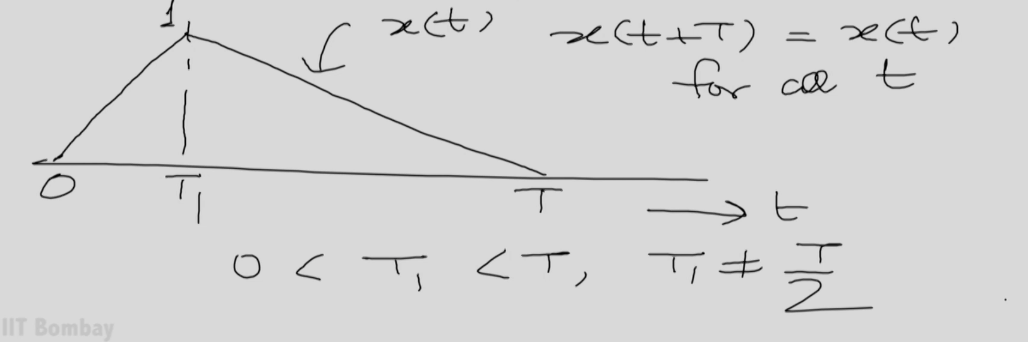
\includegraphics[scale=0.32]{S_217_5.PNG}
\end{figure}








                



                     
